	
\section{प्रस्तावना}


	रक्त में ऑक्सीजन की एकाग्रता (ऑक्सीजन संतृप्ति - SpO\textsubscript{2}) को मापने कि प्रक्रिया ओक्सिमेट्री है। SpO\textsubscript{2} रक्त में घुला ऑक्सीजन की मात्रा का मापन है। SpO\textsubscript{2} का सामान्य स्तर आमतौर पर 95\% से 100\% होना चाहिए, स्तर के 90\% से कम होने पर Hypoxemia होता है जिससे साँस की तकलीफ और सिर दर्द हो सकता है
	\footnote{\url{https://www.mayoclinic.org/symptoms/hypoxemia/basics/definition/sym-20050930}}.

\subsection{हृदय चक्र}

	रक्त की लाल कोशिका में हीमोग्लोबिन नामक प्रोटीन होता है। यह फेफड़ों से निवेश ताजा ऑक्सीजन के समपर्क मे आकर आक्सीहीमोग्लोबिन (HbO\textsubscript{2}) का उत्पाद करता है। यह रक्त फेफड़ों से दिल के बांई ओर ले जाया जाता है, जो धमनियों के माध्यम से रक्त शरीर के चारों ओर पंप करता है।
	शरीर कि कोशिका इस रक्त की लाल कोशिका मे आक्सीजन अणुओं से रासायनिक ऊर्जा को एडेनोसिन ट्राइफॉस्फेट (ATP) मे परिवर्तित
	करती है। ATP कोशिका मे संग्रहीत रहता है और आवश्यकता अनुसर जीव कि प्रक्रियाओं के लिए इस्तेमाल किया जा सकता है। इस आक्सीजन के ATP मे परिवर्तित हो जाने से डीऑक्सीजनेट हीमोग्लोबिन (Hb) बनता है।

	यह बिन ऑक्सीजन का रक्त दिल के दाईं ओर नसों के माध्यम से लौटता है, वहा से रक्त को फेफड़ों में पंप किया जाता है ताकि कार्बन डाइऑक्साइड को बाहर निकाल सकें, और फ़िर्से फेफड़ों के मधयम से रक्त मे ताजा आक्सीजन आ सके - यह एक पुर्न हृदय चक्र है।
\subsection{ओक्सिमेट्री सिद्धांत}

	पल्स ऑक्सीमीटर फोटोप्लेथीस्मोग्राफी (PPG) के सिद्धांत पर काम करता है। PPG एक ऑप्टिकल तकनीक है जिसके तहत रक्त में वॉल्यूमेट्रिक परिवर्तनों का पता लगाया जा सकता है प्रकाश स्रोत के उपयोग से। हीमोग्लोबिन मे आक्सीजन कि मात्रा अनुसार प्रकाश का अवशोषण बदलता है। इस अवशोषण मे बदलाव से ही आक्सीजन कि मात्रा मापी जा सकती है। पता लगाया गया है कि HbO\textsubscript{2} का अवशोषण इन्फ़रा-रेड (900nm) रोशनी के प्रति जादा है, जबकि Hb का अवशोषण लाल रोशनी (700nm) के प्रति जादा है (चित्र \ref{fig:spectrum})।
	यदि हम ज्ञात आउटपुट को रक्त में Hb/HbO\textsubscript{2} की सांद्रता के साथ जोड़ सके , तो SpO\textsubscript{2} की गणना करने के लिए एक समीकरण प्राप्त किया जा सकता है।

	\begin{english}
	\begin{figure}[ht!]
		\centering
		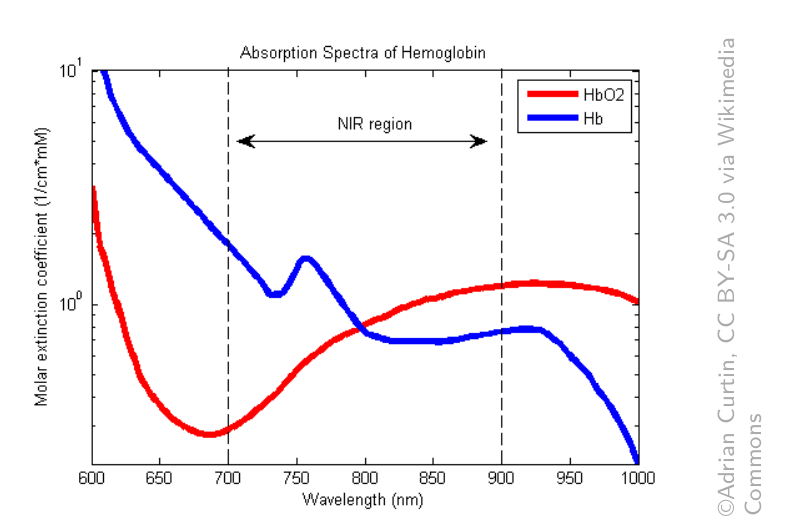
\includegraphics[width=0.7\textwidth]{../common/spectra.png}
		\caption{अवशोषण स्पेक्ट्रा - Hb व HbO\textsubscript{2}}
		\label{fig:spectrum}
	\end{figure}
	\end{english}
	
	
	\begin{figure}[ht!]
		\centering
		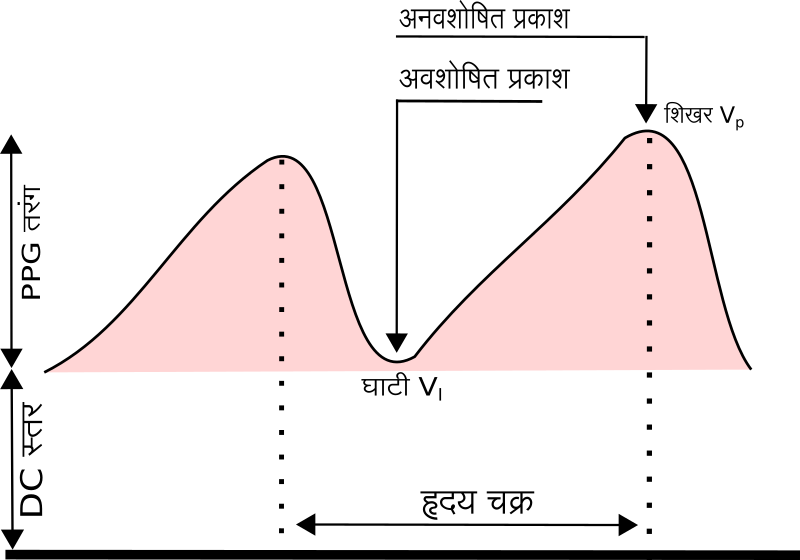
\includegraphics[width=0.7\textwidth]{images/PPG_hi.png}
		\caption{PPG तरंग - एकल प्रकाश स्रोत के प्रक्षेपित }
		\label{fig:ppg}
	\end{figure}


	हृदय रक्त पंप करता है और इससे धमनी में रक्त की मात्रा में परिवर्तन होता है प्रत्येक हृदय चक्र के साथ। जब प्रकाश (उंगली, इयरलोब, कलाई) से पारित करी जाती है, Hb/HbO\textsubscript{2} अवशोषित हो जाएँगे और PPG सिग्नल आउटपुट के रूप में प्राप्त होता है (चित्र \ref{fig:ppg})। सिग्नल शिखर एक हृदय चक्र (दिल की धड़कन) के पूरा होने का संकेत है। त्वचा, शिरापरक रक्त और ऊतक द्वारा प्रकाश स्रोत से अवशोषण के कारण इस भिन्न संकेत में DC स्तर भी होता है।.
	
	इस समझ से, यदि हम एक परिभाषित रक्त मात्रा में Hb और HbO\textsubscript{2} की आणविक सांद्रता प्रापत कर सके, तो SpO\textsubscript{2} की गणना ऑक्सीजन युक्त रक्त एकाग्रता व कुल एकाग्रता के अनुपात के रूप में की जा सकती है:
	
	\begin{equation}
		SpO\textsubscript{2} = \frac{HbO\textsubscript{2}}{Hb + 	HbO\textsubscript{2}}
	\end{equation}
	
	बियर-लैम्बर्ट नियम के अनुसार:
	
	\begin{equation}		
		\log_{10}\frac{I}{I_o} = \epsilon l c
	\end{equation}	
	
	$I -$ संचारित प्रकाश की तीव्रता
	
	$I\textsubscript{o}-$ प्रारंभिक प्रकाश की तीव्रता

	$l -$ लंबाई
	
	$c -$ अणु कि एकाग्रता
	
	$\epsilon -$ मोलर अवशोषण गुणांक\par
	\medskip
	
	\begin{figure}[ht!]
		\centering
		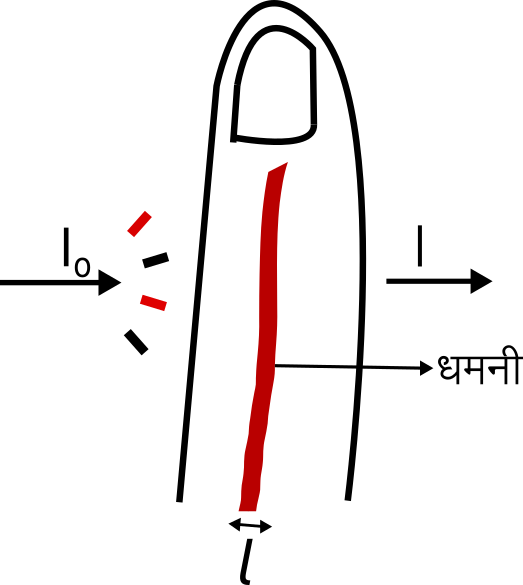
\includegraphics[width=0.3\textwidth]{images/finger_hi.png}
		\caption{उंगली पर प्रक्षेपित प्रकाश स्रोत}
		\label{fig:finger}
	\end{figure}
	
	जैसा कि चित्र \ref{fig:finger} मे देखा जा सकता है, एक प्रकाश स्रोत को उंगली पर दर्शाया गया है।
	2 तरीके के प्रकाश सौत्र बारी-बारी से प्रकाशित किए गये है। उंगली के अलावा ईयरलोब/माथा/कलाई पर भी सौत्र दर्शाया जा सकता है। इन्फ़रा-रेड स्रोत के लिये नियम अनुसार:
	
	\[	
	c_1 = 	\frac{\log_{10}\frac{I_1}{I_{o1}}}{\epsilon_1 l}
	\]	
	
	इन्फ़रा-रेड स्रोत से HbO\textsubscript{2} का अवशोषण जादा होता है, यह मानते हुये,
	
	\[	
	HbO_2 = \frac{\log_{10}\frac{I_1}{I_{o1}}}{\epsilon_1 	l}
	\]	
	
	उसी धारणा का उपयोग करते हुए लाल स्रोत के लिये,
	\[	
	Hb = \frac{\log_{10}\frac{I_2}{I_{o2}}}{\epsilon_2 	l}
	\]
	
	(1) के अनुसार,
	
	\[	
	SpO_2 =  \frac{\frac{\log_{10}\frac{I_1}{I_{o1}}}{\epsilon_1 l}}		
	{\frac{\log_{10}\frac{I_2}{I_{o2}}}{\epsilon_2 l} + 	\frac{\log_{10}\frac{I_1}{I{o1}}}{\epsilon_1 l}}
	\]	
	
	यदि $R = \frac{\log_{10}\frac{I_2}{I_{o2}}}{\log_{10}\frac{I_1}{I_{o1}}}$,
	
	\[	
	SpO_2 = \frac{\frac{1}{\epsilon_1}}{\frac{R}{\epsilon_2} + \frac{1}{\epsilon_1}}
	\]	
	
	\begin{equation}
		SpO_2 = \frac{\epsilon_2}{R\epsilon_1 + \epsilon_2}
	\end{equation}	
	
	
	SpO\textsubscript{2} ज्यादातर R पर निर्भर करता है, हम R की गणना कर सकते हैं और बाद में वास्तविक SpO\textsubscript{2} प्राप्त करने के लिए कैलिब्रेटेड संदर्भ के साथ तुलना कर सकते हैं।
	
	चूंकि स्पंदित होने पर प्रारम्भिक प्रकाश की तीव्रता का स्तर स्थिर रहेगा, R केवल I\textsubscript{1} और I\textsubscript{2} पर निर्भर करेगा,
	
	\[
	R \approx \frac{\log_{10}{I_2}}{\log_{10}{I_1}} \approx \frac{I_2}{I_1} \approx \frac{AC_2}{AC_1}
	\]				
	
	हमें लघुगणक की गणना करने की आवश्यकता नहीं है, क्योंकि वास्तविक SpO\textsubscript{2} एक लुक अप तालिका से प्राप्त की जाएगी जिसमें R व SpO\textsubscript{2} का संख्यात्मक संबंध शामिल होगा। ऑक्सीमीटर निर्माता आमतौर पर विभिन्न तरह के लोगो पर अपने ऑक्सीमीटर का परीक्षण करते हैं (R की गणना) और एक अलग कैलिब्रेटेड मीटर का उपयोग करके व्यक्ति का वास्तविक SpO\textsubscript{2} प्राप्त करते है। यह संख्यात्मक संबंध R व SpO\textsubscript{2} का प्राप्त हो जाने पर, किसी भी व्यक्ति के लिए SpO\textsubscript{2} की गणना तुलना करके मापी जा सकती है।
	
	\begin{figure}[ht!]
	\centering	
	\begin{tikzpicture}
		\begin{axis}[
			xlabel = R,
			ylabel = SpO\textsubscript{2}\%]
			\addplot coordinates {
				(0.4, 100)
				(1, 85)
				(1.5, 72.5)
				(2, 60)
				(2.5, 47.5)
				(3, 35)
				(3.5, 22.5)
				(4, 10)
				(4.4,0)
			};
			
		\end{axis}
	\end{tikzpicture}
	\caption{एक विशिष्ट संबंध वक्र R vs SpO\textsubscript{2}}
	\label{fig:curve}
	\end{figure}
	
	लाल और इन्फ़्रा-रेड सिग्नल में DC स्तर अलग-अलग हो सकते हैं, हमें पहले DC स्तरों को विभाजित करके अनुपात को सामान्य करना होगा ताकि PPG (AC घटक) की सीधी तुलना की जा सके क्योंकि इसमें अवशोषित/अन-अवशोषित जानकारी होती है। R अब बन जाता है:
	
	
	\[
		R = \sfrac{\frac{AC_2}{DC_2}}{{\frac{AC_1}{DC_1}}}
	\]	
	

	\begin{figure}[ht!]
	\centering
	\subfloat[सामान्यीकरण से पहले
	]{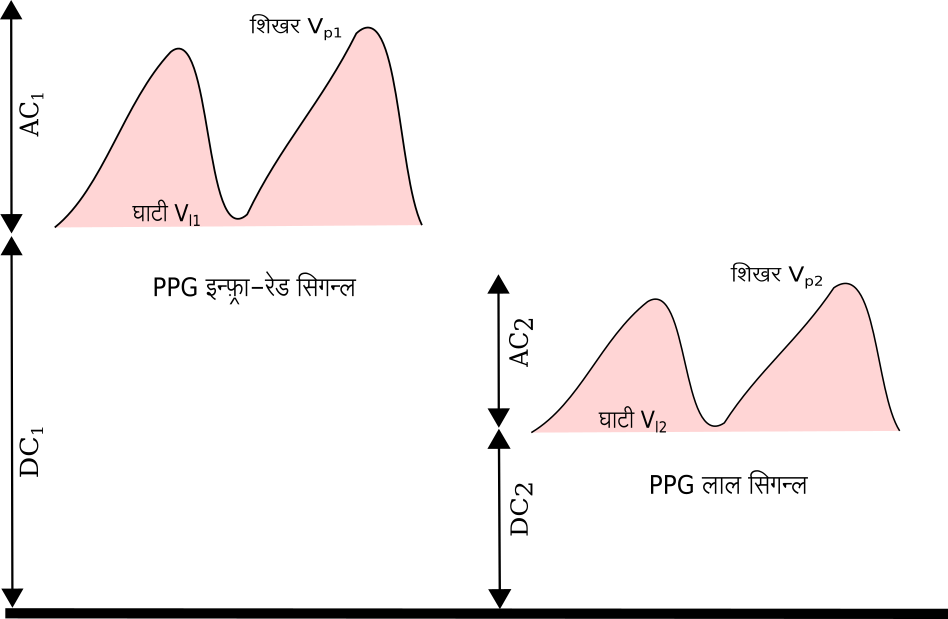
\includegraphics[width=0.7\textwidth]{images/PPG_norm1.png}}
	\hfill
	\subfloat[सामान्यीकरण के बाद
	]{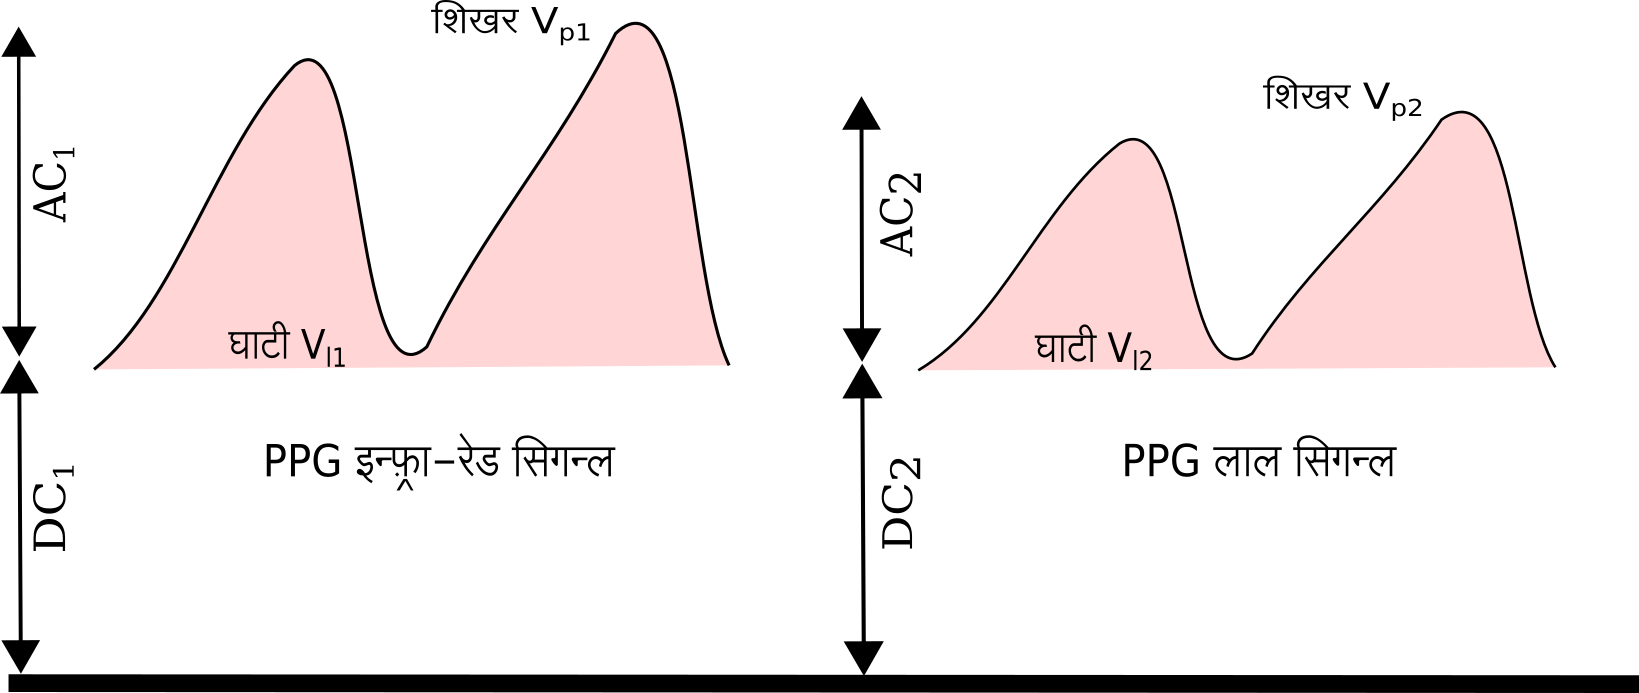
\includegraphics[width=0.7\textwidth]{images/PPG_norm2.png}}
	\caption{सामान्यीकरण का प्रभाव}
	\label{fig:ppgnorm}
	\end{figure}

	\begin{equation}
	\label{eq:calc}	
	R = \sfrac{\frac{V_{p2} - V_{l2}}{DC_2}}{\frac{V_{p1} - V_{l1}}{DC_1}}
	\end{equation}	 
	
	चित्र \ref{fig:ppgnorm} के अनुसार,
	
	$V_{p1} - $  इन्फ़्रारेड शिखर
	
	$V_{l1} - $  इन्फ़्रारेड घाटी
	
	$V_{p2} - $  लाल शिखर
	
	$V_{l2} - $  लाल शिखर
	
	$DC_1 - $  इन्फ़्रारेड DC स्तर
	
	$DC_2 - $  लाल DC स्तर
	
	\medskip
	
	हम R की गणना के लिये पड़ोसी समंक बिन्दुओं का इस्तिमाल करने पर विचार कर सक़ते हैं और उनका औसत निकाल सक़ते है बजाए कि चोटियों और घाटियों के आने की प्रतीक्षा करे। पड़ोसी समंक बिन्दुओं के बीच एक भारित औसत \cite{wuk} की गणना अंतिम मान के लिए की जाती है। इस पर आगे SpO\textsubscript{2} ऐल्गोरिद्म अनुभाग में चर्चा की गई है।
	
